\documentclass[tikz,border=2pt]{standalone}
\usepackage{amsmath}
\usetikzlibrary{arrows.meta}
\begin{document}
% A = [[1,1],[1,1]], b = (2,2)^T: the generalized inverses G = diag(1,0) and G' = diag(0,1) give
% different particular solutions Gb = (2,0)^T and G'b = (0,2)^T, but both lie on the same solution set
% x_1 + x_2 = 2, which is Gb + (I - GA)z with (I - GA)z = z_2(-1,1)^T.
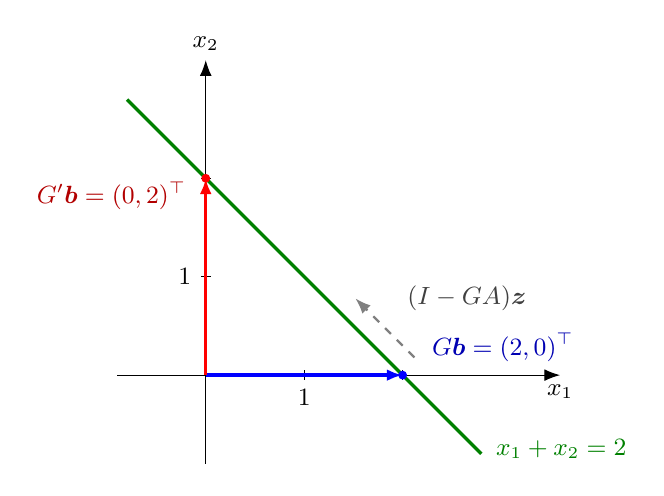
\begin{tikzpicture}[font=\small, >={Latex[length=2mm]}, x=1.25cm, y=1.25cm]
  \draw[->] (-0.9,0) -- (3.6,0) node[below] {$x_1$};
  \draw[->] (0,-0.9) -- (0,3.2) node[above] {$x_2$};
  \foreach \k in {1,2} {
    \draw (\k,0.05) -- (\k,-0.05);
    \draw (0.05,\k) -- (-0.05,\k);
  }
  \node[below] at (1,-0.05) {$1$};
  \node[left] at (-0.05,1) {$1$};
  % solution set
  \draw[green!50!black, very thick] (-0.8,2.8) -- (2.8,-0.8);
  \node[green!50!black, anchor=west] at (2.85,-0.75) {$x_1+x_2=2$};
  % particular solutions from two generalized inverses
  \draw[->, blue, very thick] (0,0) -- (2,0);
  \fill[blue] (2,0) circle (1.6pt);
  \node[blue!70!black, anchor=south west] at (2.2,0.04) {$G\boldsymbol{b}=(2,0)^{\top}$};
  \draw[->, red, very thick] (0,0) -- (0,2);
  \fill[red] (0,2) circle (1.6pt);
  \node[red!70!black, anchor=east] at (-0.1,1.82) {$G'\boldsymbol{b}=(0,2)^{\top}$};
  % homogeneous direction
  \draw[->, gray, thick, dashed] (2.12,0.18) -- (1.52,0.78);
  \node[gray!50!black, anchor=south west] at (1.95,0.55) {$(I-GA)\boldsymbol{z}$};
\end{tikzpicture}
\end{document}
